\documentclass{article}
\usepackage[margin=3cm]{geometry}
\usepackage[utf8]{inputenc}
\usepackage{amsmath}
\usepackage{amssymb}
\usepackage{float}
\usepackage{enumitem}
\usepackage{graphicx}
\usepackage{caption}
\usepackage{subcaption}

\graphicspath{ {plots/} }

\title{Nonlinear Optimization - Homework 2 }
\author{Christian Segercrantz 481056}


\begin{document}
\maketitle
\pagebreak
\section*{3.1}
	\begin{alignat}{2}
		\text{min. } & -x_1 \\
		\text{subject to: } & x_2 \leq (1-x_1)^3 \label{eq:3.1_g1}\\
		&x_1 \geq 0 \\
		& x_2 \geq 0
	\end{alignat}
	\begin{figure}[H]
		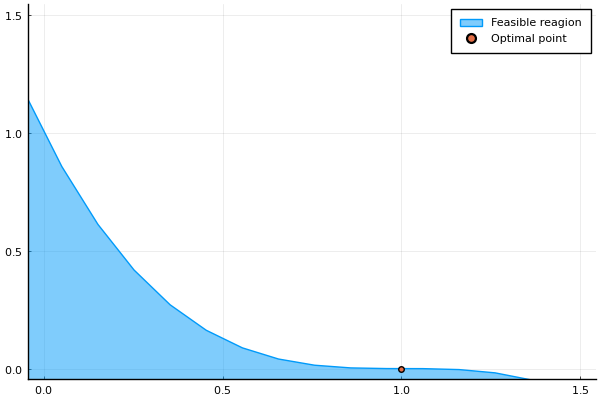
\includegraphics[width=0.8\textwidth]{3_1.png}
		\caption{The feasible region of the problem of exercise 3.1. The condition of $x_1$,$x_2\geq 0$ is implemented by the limits of the plot.}
		\label{fig:1a}
	\end{figure}
	Figure \ref{fig:1a} shows the feasible region for the problem above. Since minimizing $-x_1$ is the same as maximizing $x_1$, we can identify the optimal point as $\bar{x} = \begin{bmatrix} 1 \\ 0 \end{bmatrix}$.
	
	We will change around Equation \ref{eq:3.1_g1} to be $(1-x_1)^3-x_2 \geq 0$ for it to fit into the FJ conditions. 
	
	\begin{align}
		0 &= u_0 \nabla f(\bar{x}) + \sum_{i=1}^{m} u_i \nabla g_i(\bar{x}) \\
		0 &= u_0 (-1 \begin{bmatrix} 1 \\ 0 \end{bmatrix}) + u_1 \begin{bmatrix}3(1-x_1)^2 \\ -1 \end{bmatrix} + u_2 \begin{bmatrix} 1 \\ 0 \end{bmatrix} + u_3 \begin{bmatrix} 0 \\ 1 \end{bmatrix} \\
		0 &= u_0 ( \begin{bmatrix} -1 \\ 0 \end{bmatrix}) + u_1 \begin{bmatrix} 0 \\ -1 \end{bmatrix} + u_2 \begin{bmatrix} 1 \\ 0 \end{bmatrix} + u_3 \begin{bmatrix} 0 \\ 1 \end{bmatrix} \\
		0 &= \begin{bmatrix}
			-u_0+u_2 \\
			-u_1+u_3
		\end{bmatrix}\\
		\implies & \begin{cases}
			u_0 = u_2 \\
			u_1 = u_3
		\end{cases}		
	\end{align}
\section*{3.2}
\subsection*{a)}
	\begin{alignat}{2}
		\text{min. } & (x_1 +\frac{9}{4})^2 + (x_2 - 2)^2 \\
		\text{subject to: } & x_2-x_1^2 \geq 0\\
		& x_1 + x_2 \leq 6\\
		& x_1 \geq 0\\
		& x_2 \geq 0		
	\end{alignat}
	The KKT conditions for the problem is
	\begin{align}
		0 = & \nabla f(\bar{x}) + \sum_{i=1}^{m} u_i \nabla g_i(\bar{x})\\
		0 = & \begin{bmatrix} 2(\bar{x}_1 +\frac{9}{4}) \\ 2(\bar{x}_2 -2)\end{bmatrix} + u_1 \begin{bmatrix} -2\bar{x}_1 \\ 1 \end{bmatrix} + u_2 \begin{bmatrix} -1 \\ -1 \end{bmatrix} + u_3 \begin{bmatrix} 1 \\ 0 \end{bmatrix} + u_4 \begin{bmatrix} 0 \\ 1 \end{bmatrix}\\
		0 = & \begin{bmatrix} 2(\frac{3}{2} +\frac{9}{4}) \\ 2(\frac{9}{4} -2)\end{bmatrix} + u_1 \begin{bmatrix} -2\frac{3}{2} \\ 1 \end{bmatrix} + u_2 \begin{bmatrix} -1 \\ -1 \end{bmatrix} + u_3 \begin{bmatrix} 1 \\ 0 \end{bmatrix} + u_4 \begin{bmatrix} 0 \\ 1 \end{bmatrix} \\
		0 = & \begin{bmatrix}2(\frac{3}{2} +\frac{9}{4}) -\frac{7}{2}u_1 - u_2 +u_3 \\ 2(\frac{9}{4} -2) +u_1 -u_2 +u_4
		 \end{bmatrix}
	\end{align}
\subsection*{b)}
	\begin{figure}[H]
		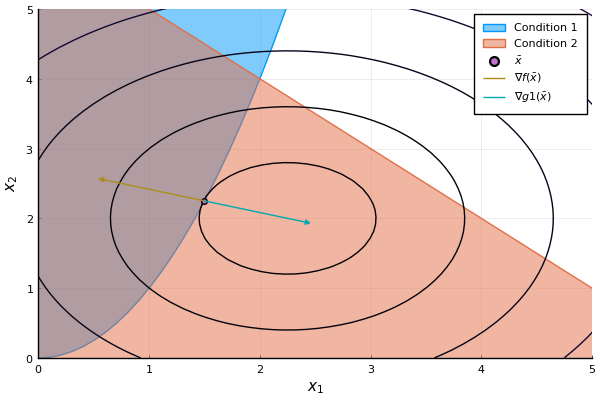
\includegraphics[width=0.8\textwidth]{3_2.png}
		\caption{}
		\label{fig:2a}
	\end{figure}
\end{document}